%

\label{chap:intro}
\paragraph{}
At the outset of this project we had several goals in mind. These included learning more about how to implement distributed primitives in the future, learning more about how to design these primitives with tiling in mind, and the actual development of two performant, distributed matrix multiplication algorithms. With respect to the first goal we now know that distributed primitives may need auxiliary data structures to support efficient organization of tiling information, and that writing distributed primitives is a process that is uniquely challenging, in a way that serial primitives is not. With respect to auxiliary data structures, an example is how we were required to construct a representation of the tile row from the annotation for the LHS operand and a representation of the tile column for the RHS operand in the Cannon Product. This is directly related to how the Cannon Product runs, and other algorithms may need their own tailored way of traversing existing tiling. In the case of dot\_d, we did not need an extra data structure for execution aside from the existing annotations. With respect to the second goal we learned that for tiling analysis with the goal of optimization, uniform tiling is much simpler to work with than non-uniform tiling. For the last goal, we produced two algorithms for matrix multiplication, as we set out to.
\section{Results}
With the two matrix multiplication algorithms completed, we were able to run some preliminary performance tests. Table \ref{table_1} displays those results in tabular form, and figure \ref{Fig_10} displays them in a graph. In figure \ref{Fig_11} we can see the speedup achieved by the respective algorithms, calculated as $Speedup = t_1/t_N$ where $t_1$ is the time in the single process version and $t_N$ is the version with $N$ processes. In our case, as they are only preliminary results, we only tested on 1 process, and on 4 processes. We obtained these results running the application with 4 separate processes on a single Windows machine, versus a single process for the linear version. Due to unexpected technical complications, we were not able to use the threading ordinarily used in the Blaze linear algebra library for our tests. Although our tests were performed in a shared memory environment, and thus could be contested, we believe that the requirement of communicating through the TCP/IP layer in HPX means that the results are approximately equivalent to running in a fully distributed environment. In the tests we ran, we found that the Cannon product was always the fastest, achieving a speed-up relative to the serial of between $~2.6$ and $~3.2$. Cannon consistently outperformed dot\_d. As we mentioned before, we believe that the lack of a reduction step across tile rows in the output matrix substantially aided the Cannon product, as well as its use of futurization of the fetches. Of course, further testing is required to confirm these results.


\begin{table}
	\centering
	\begin{tabular}{|c|c|c|c|} 
		\hline
		Matrix Size & dot\_d & Cannon & dot (serial) \\ [0.5ex] 
		\hline
		500 & 5351.08 & 3131.345 & 8538.37 \\ 
		\hline
		1000 & 26946.15 & 25889.2 & 67425.2 \\
		\hline
		2000 & 282916.5 & 170091.5 & 539491 \\ [1ex]
		\hline
	\end{tabular}
	\caption{Preliminary Test Results}
	\label{table_1}
\end{table}

\begin{figure}
	\centering
	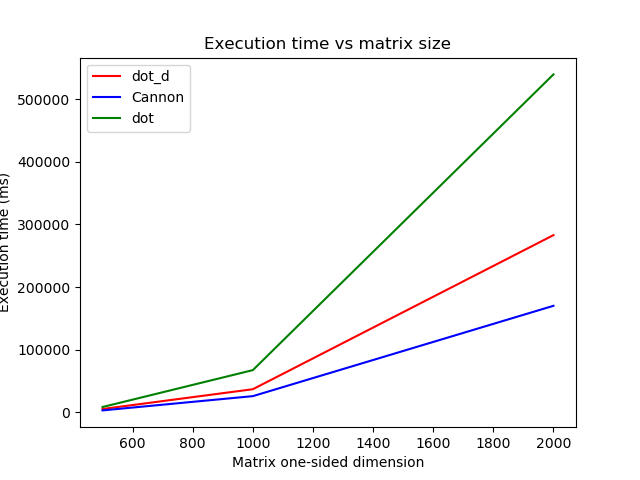
\includegraphics[width=150mm]{performance_comparison}
	\caption{Preliminary Test Results - Raw timings}
	\label{Fig_10}
\end{figure}

\begin{figure}
	\centering
	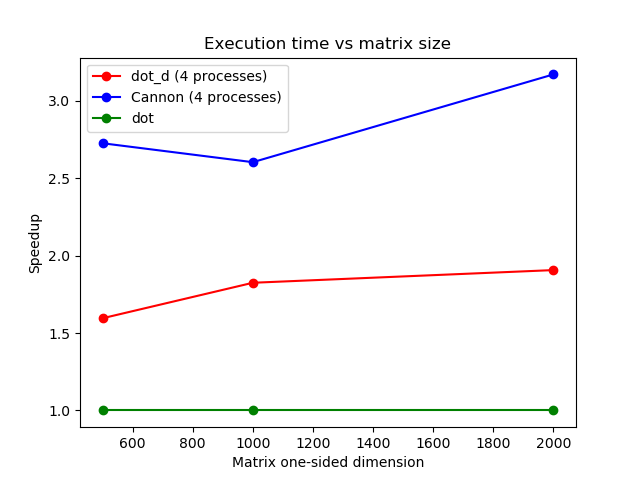
\includegraphics[width=150mm]{speed_up_plot}
	\caption{Preliminary Test Results - Speedup}
	\label{Fig_11}
\end{figure}

\section{Future work}
Although these results are only preliminary, they are encouraging, and suggest that our work on this project has meaningfully advanced the state of the Phylanx project. In order to advance closer to having a robust system for performing linear algebra for ML applications, or otherwise, we have several new objectives. The main one is in expanding our lineup of distributed primitives, to allow for something of a "distributed computational basis" for ML applications. This necessitates functionality like distributed add/map, distributed file read/write, and other linear algebra primitives like matrix inverse, and matrix factorization. We also would like to be able to use this system to aid in providing testing data for the tiling optimization facet of Phylanx. The capacity to write many different algorithms with different tilings, and extract performance data will help give intuition, or experimental validation, in the development of a static tiling optimizer.
	



%
